\documentclass[10pt]{article}
\usepackage{float}
\RequirePackage{eso-pic}
\usepackage{caption}
\captionsetup[table]{labelformat=empty}



\usepackage{geometry}
\geometry{
a4paper,
left=11mm,
right=14mm,
top=37mm,
bottom=14mm,
}



\usepackage{colortbl}
\usepackage{fontspec}
\setmainfont[Ligatures=TeX]{Calibri}



\newcommand\BackgroundPic{%
\put(0,0){%
\parbox[b][\paperheight]{\paperwidth}{%
\vfill
\centering
\includegraphics{MBIE_generic_background.pdf}%
\vfill
}}}



\begin{document}
\thispagestyle{empty}
\AddToShipoutPicture{\BackgroundPic}
\section*{Key Export Statistics\footnotemark - Sugar Confectionery\footnotemark }
\today\\
\begin{table}[ht]
\centering
{\scriptsize
\begin{tabular}[t]{p{1.8cm}>{\hfill}p{1.4cm}>{\hfill}p{1.4cm}>{\hfill}p{1.6cm}>{\hfill}p{1.9cm}>{\hfill}p{2cm}>{\hfill}p{1.9cm}>{\hfill}p{1.5cm}}
 \textbf{Country} & \textbf{Yearly Qty} & \textbf{Yearly Value} & \textbf{Yearly Price} & \textbf{3Year CAGR(Qty)} & \textbf{3Year CAGR(Value)} & \textbf{3Year CAGR(Price)} & \textbf{Price Elasticity} \\
\hline
Australia & 8,887 & 56.7 & \$6.4 & -4.9\% & -7.2\% & -2.4\% & 2.0 \\  
USA & 335 & 2.6 & \$7.8 & 21.2\% & 26.8\% & 4.6\% & 4.6 \\  
United Kingdom & 198 & 1.6 & \$8.1 & -4.8\% & 4.2\% & 9.4\% & -0.5 \\  
Hong Kong & 53 & 1.3 & \$24.9 & -8.1\% & 4.8\% & 14\% & -0.6 \\  
Poland & 5 & 0.8 & \$166.0 & -17.4\% & 144.9\% & 196.6\% & -0.1 \\  
China & 16 & 0.6 & \$41.8 & -63.7\% & -35.2\% & 78.2\% & -0.8 \\  
Other & 386 & 3.2 & \$8.2 & -67.4\% & -65.6\% & 5.6\% & -11.9 \\  
Total & 9,878 & 66.9 & \$6.8 & -1.5\% & -2\% & -0.5\% & 3.2 \\  
\hline
\end{tabular}
}
\caption{\scriptsize Top 6 Sugar Confectionery Markets for year ending November - 2015: Quantity('000 kg) Value(NZ\$Mill), Price and their last 3-Year Growth Rates}
\end{table}


\vspace{-0.7cm}



   \begin{figure}[H]
   \centering
    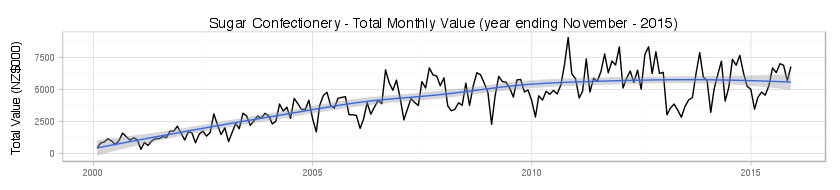
\includegraphics[scale=0.5]{../graphs/monthly_value/sugar_confectionery_monthly_value.png} \
    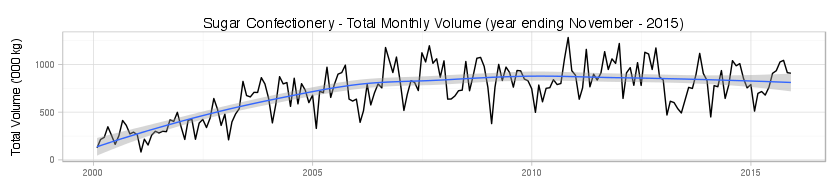
\includegraphics[scale=0.5]{../graphs/monthly_volume/sugar_confectionery_monthly_volume.png} \
    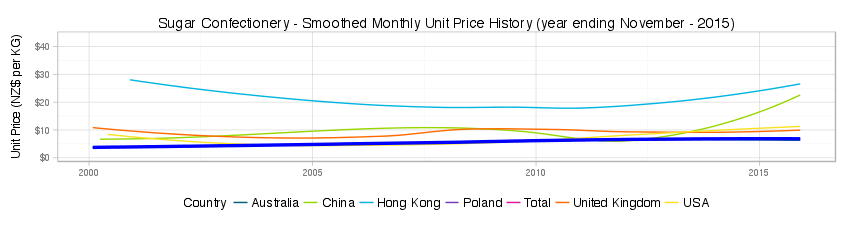
\includegraphics[scale=0.5]{../graphs/smoothed_price/sugar_confectionery_smoothed_price.png} \
    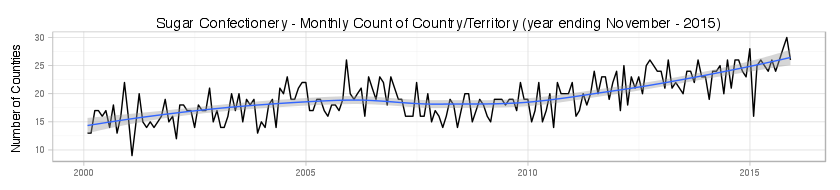
\includegraphics[scale=0.5]{../graphs/monthly_number_countries/sugar_confectionery_monthly_count.png} \
    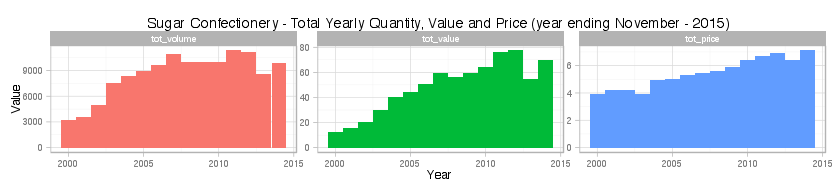
\includegraphics[scale=0.5]{../graphs/yearly_summary/sugar_confectionery_yearly_summary.png} \
   \end{figure}



\footnotetext[1]{Source: Statistics New Zealand - Overseas Merchandise Trade}
\footnotetext[2]{Harmonised System Codes for Sugar Confectionery starting with: 170490.}
\end{document}
